\documentclass[journal,12pt,twocolumn]{IEEEtran}

\usepackage{setspace}
\usepackage{gensymb}
\singlespacing
\usepackage[cmex10]{amsmath}

\usepackage{amsthm}

\usepackage{mathrsfs}
\usepackage{txfonts}
\usepackage{stfloats}
\usepackage{bm}
\usepackage{cite}
\usepackage{cases}
\usepackage{subfig}

\usepackage{longtable}
\usepackage{multirow}

\usepackage{enumitem}
\usepackage{mathtools}
\usepackage{steinmetz}
\usepackage{tikz}
\usepackage{circuitikz}
\usepackage{verbatim}
\usepackage{tfrupee}
\usepackage[breaklinks=true]{hyperref}
\usepackage{graphicx}
\usepackage{tkz-euclide}

\usetikzlibrary{calc,math}
\usepackage{listings}
    \usepackage{color}                                            %%
    \usepackage{array}                                            %%
    \usepackage{longtable}                                        %%
    \usepackage{calc}                                             %%
    \usepackage{multirow}                                         %%
    \usepackage{hhline}                                           %%
    \usepackage{ifthen}                                           %%
    \usepackage{lscape}     
\usepackage{multicol}
\usepackage{chngcntr}

\DeclareMathOperator*{\Res}{Res}

\renewcommand\thesection{\arabic{section}}
\renewcommand\thesubsection{\thesection.\arabic{subsection}}
\renewcommand\thesubsubsection{\thesubsection.\arabic{subsubsection}}

\renewcommand\thesectiondis{\arabic{section}}
\renewcommand\thesubsectiondis{\thesectiondis.\arabic{subsection}}
\renewcommand\thesubsubsectiondis{\thesubsectiondis.\arabic{subsubsection}}


\hyphenation{op-tical net-works semi-conduc-tor}
\def\inputGnumericTable{}                                 %%

\lstset{
%language=C,
frame=single, 
breaklines=true,
columns=fullflexible
}
\begin{document}


\newtheorem{theorem}{Theorem}[section]
\newtheorem{problem}{Problem}
\newtheorem{proposition}{Proposition}[section]
\newtheorem{lemma}{Lemma}[section]
\newtheorem{corollary}[theorem]{Corollary}
\newtheorem{example}{Example}[section]
\newtheorem{definition}[problem]{Definition}

\newcommand{\BEQA}{\begin{eqnarray}}
\newcommand{\EEQA}{\end{eqnarray}}
\newcommand{\define}{\stackrel{\triangle}{=}}
\bibliographystyle{IEEEtran}
\raggedbottom
\setlength{\parindent}{0pt}
\providecommand{\mbf}{\mathbf}
\providecommand{\pr}[1]{\ensuremath{\Pr\left(#1\right)}}
\providecommand{\qfunc}[1]{\ensuremath{Q\left(#1\right)}}
\providecommand{\sbrak}[1]{\ensuremath{{}\left[#1\right]}}
\providecommand{\lsbrak}[1]{\ensuremath{{}\left[#1\right.}}
\providecommand{\rsbrak}[1]{\ensuremath{{}\left.#1\right]}}
\providecommand{\brak}[1]{\ensuremath{\left(#1\right)}}
\providecommand{\lbrak}[1]{\ensuremath{\left(#1\right.}}
\providecommand{\rbrak}[1]{\ensuremath{\left.#1\right)}}
\providecommand{\cbrak}[1]{\ensuremath{\left\{#1\right\}}}
\providecommand{\lcbrak}[1]{\ensuremath{\left\{#1\right.}}
\providecommand{\rcbrak}[1]{\ensuremath{\left.#1\right\}}}
\theoremstyle{remark}
\newtheorem{rem}{Remark}
\newcommand{\sgn}{\mathop{\mathrm{sgn}}}
\providecommand{\abs}[1]{\left\vert#1\right\vert}
\providecommand{\res}[1]{\Res\displaylimits_{#1}} 
\providecommand{\norm}[1]{\left\lVert#1\right\rVert}
%\providecommand{\norm}[1]{\lVert#1\rVert}
\providecommand{\mtx}[1]{\mathbf{#1}}
\providecommand{\mean}[1]{E\left[ #1 \right]}
\providecommand{\fourier}{\overset{\mathcal{F}}{ \rightleftharpoons}}
%\providecommand{\hilbert}{\overset{\mathcal{H}}{ \rightleftharpoons}}
\providecommand{\system}{\overset{\mathcal{H}}{ \longleftrightarrow}}
	%\newcommand{\solution}[2]{\textbf{Solution:}{#1}}
\newcommand{\solution}{\noindent \textbf{Solution: }}
\newcommand{\cosec}{\,\text{cosec}\,}
\providecommand{\dec}[2]{\ensuremath{\overset{#1}{\underset{#2}{\gtrless}}}}
\newcommand{\myvec}[1]{\ensuremath{\begin{pmatrix}#1\end{pmatrix}}}
\newcommand{\mydet}[1]{\ensuremath{\begin{vmatrix}#1\end{vmatrix}}}
\numberwithin{equation}{subsection}
\makeatletter
\@addtoreset{figure}{problem}
\makeatother
\let\StandardTheFigure\thefigure
\let\vec\mathbf
\renewcommand{\thefigure}{\theproblem}
\def\putbox#1#2#3{\makebox[0in][l]{\makebox[#1][l]{}\raisebox{\baselineskip}[0in][0in]{\raisebox{#2}[0in][0in]{#3}}}}
     \def\rightbox#1{\makebox[0in][r]{#1}}
     \def\centbox#1{\makebox[0in]{#1}}
     \def\topbox#1{\raisebox{-\baselineskip}[0in][0in]{#1}}
     \def\midbox#1{\raisebox{-0.5\baselineskip}[0in][0in]{#1}}
\vspace{3cm}
\title{AI5002: Binomial Assignment}
\author{Debolena Basak\\ AI20RESCH11003}
\maketitle
\newpage
\bigskip
\renewcommand{\thefigure}{\theenumi}
\renewcommand{\thetable}{\theenumi}
Download all Python codes from 
\begin{lstlisting}
https://github.com/Debolena/AI5002-Probability-and-Random-Variables/blob/main/compulsory%20binomial%20assignment/binomial_simulation.py
\end{lstlisting}
%
and latex-tikz codes from 
%
\begin{lstlisting}
https://github.com/Debolena/AI5002-Probability-and-Random-Variables/blob/main/compulsory%20binomial%20assignment/latex.tex
\end{lstlisting}
\section{Problem}
Let, $X_1 \sim Bin(n_1, p)$ and $X_2 \sim Bin(n_2, q)$, independently. Find the PMF of $X_1 - X_2.$
\section{Solution}
Given, $X_1 \sim Bin(n_1, p)$ and $X_2 \sim Bin(n_2, q)$, independently.\\
$\therefore n_2-X_2 \sim Bin(n_2, p)$\\
By additive/ reproductive property of binomial,\\
$X_1+n_2-X_2 \sim Bin(n_1+n_2, p)$\\
Let, $D= X_1 -X_2$.
\begin{align}
    P(D=d) &= P(X_1 -X_2 = d)\\
    &= P(X_1 -X_2 +n_2 = d +n_2)\\
    &= \binom{n_1+n_2}{n_2+d} p^{n_2+d} q^{n_1-d}, d= -n_2\ \text{to}\ n_1\ \label{subtraction}
\end{align}
\section{Reproductive property}
If $X_1 \sim  Bin(n_1, p)$ and $X_2 \sim Bin(n_2, p)$, then\\
$Y= X_1 + X_2 \sim Bin(n_1+n_2, p)$.
\section{Proof}
Let, $X_1 \sim  Bin(n_1, p)$ and $X_2 \sim Bin(n_2, p)$\\
Then, $Y= X_1 + X_2$ takes values 0,1,2,....,$\brak{n_1+n_2} $
\begin{align}
    &P(Y=y) , y=0,1,2,...,\brak{n_1+n_2}\\
    &= P(X_1+X_2 = y)\\
    &= \sum_{x_1=0}^{min\brak{n_1,y}} P(X_1=x_1, X_2= y-x_1)\\
    &= \sum_{x_1=0}^m P(X_1=x_1). P(X_2= y-x_1), m=min(n_1,y)\\
    &= \sum_{x_1=0}^m \binom{n_1}{x_1}p^{x_1} q^{n_1 - x_1}. \binom{n_2}{y-x_1} p^{y-x_1} q^{n_2-y+x_1}\\
    &= p^y.q^{n_1+n_2-y}. \sum_{x_1=0}^m \binom{n_1}{x_1} \binom{n_2}{y-x_1}\\
    &= \binom{n_1+n_2}{y}. p^y.q^{n_1+n_2-y}
\end{align}
$\therefore \quad Y= X_1+X_2 \sim Bin(n_1+n_2, p)$
\section{Problem}
Let X represent the difference between the
number of heads and the number of tails
obtained when a coin is tossed 6 times. What
are possible values of X?
\section{Solution}
Let $U_1$ denotes the number of heads and $U_2$ denotes the number of tails that occur when a coin is tossed 6 times.\\
Clearly, $U_1 \sim Bin(n=6, p)$\\
and $U_2 \sim Bin(n=6,1-p=q)$.\\
$\therefore n-U_2 \sim Bin(6, p)$.\\
By reproductive property,
\begin{align}
    U_1+n-U_2 \sim Bin(6+6, p)
\end{align}
$X=U_1-U_2$. Using \eqref{subtraction},
\begin{align}
    P(X=x) = \binom{6+6}{6+x} p^{6+x} q^{6-x}, x= -6\ \text{to}\ 6 
\end{align}
Suppose, the coin is unbiased. Then, $p=q= \frac{1}{2}$.
\begin{align}
    \therefore P(X=x) = \binom{12}{6+x}\brak{\frac{1}{2}}^{12}, x= -6\ \text{to}\ 6 
\end{align}

\begin{figure}[!ht]
\centering
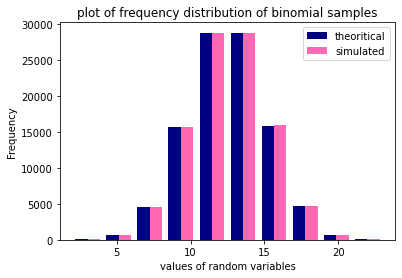
\includegraphics[width=\columnwidth]{plot_binomial.png}
\caption{Binomial Frequency plot}
\label{fig:binomial plot}
\end{figure}
\end{document}
